\chapter{Sequenzdiagramme}
Um die verschiedenen möglichen Abläufe zu verdeutlichen wurden einige Sequenzdiagramme erstellt, die die Funktionen der Anwendung einfach und effektiv zu erklären.


\begin{itemize}


    \item Der Benutzer ist mit seiner eindeutigen User ID angemeldet und will alle seine Workflows sehen (\ref{sqd_get_all_workflows}). Hierfür wird clientseitig eine Liste an Observables in einer Instanz von WorkflowService angelegt. Dann wird ein HTTP Request an die zugehörige serverseitige Instanz von view.Workflow geschickt. Diese fragt bei der Datenbank in model.Workflow die Daten an und schickt sie per HTTP Response zurück an die vorherige Instanz von WorkflowService. Hier wird anschließend die Referenz auf die Observables aktualiziert, wodurch der Benutzer jetzt alle seine Workflows angezeigt bekommt. 
    
    \begin{figure}[h]
        \centering
        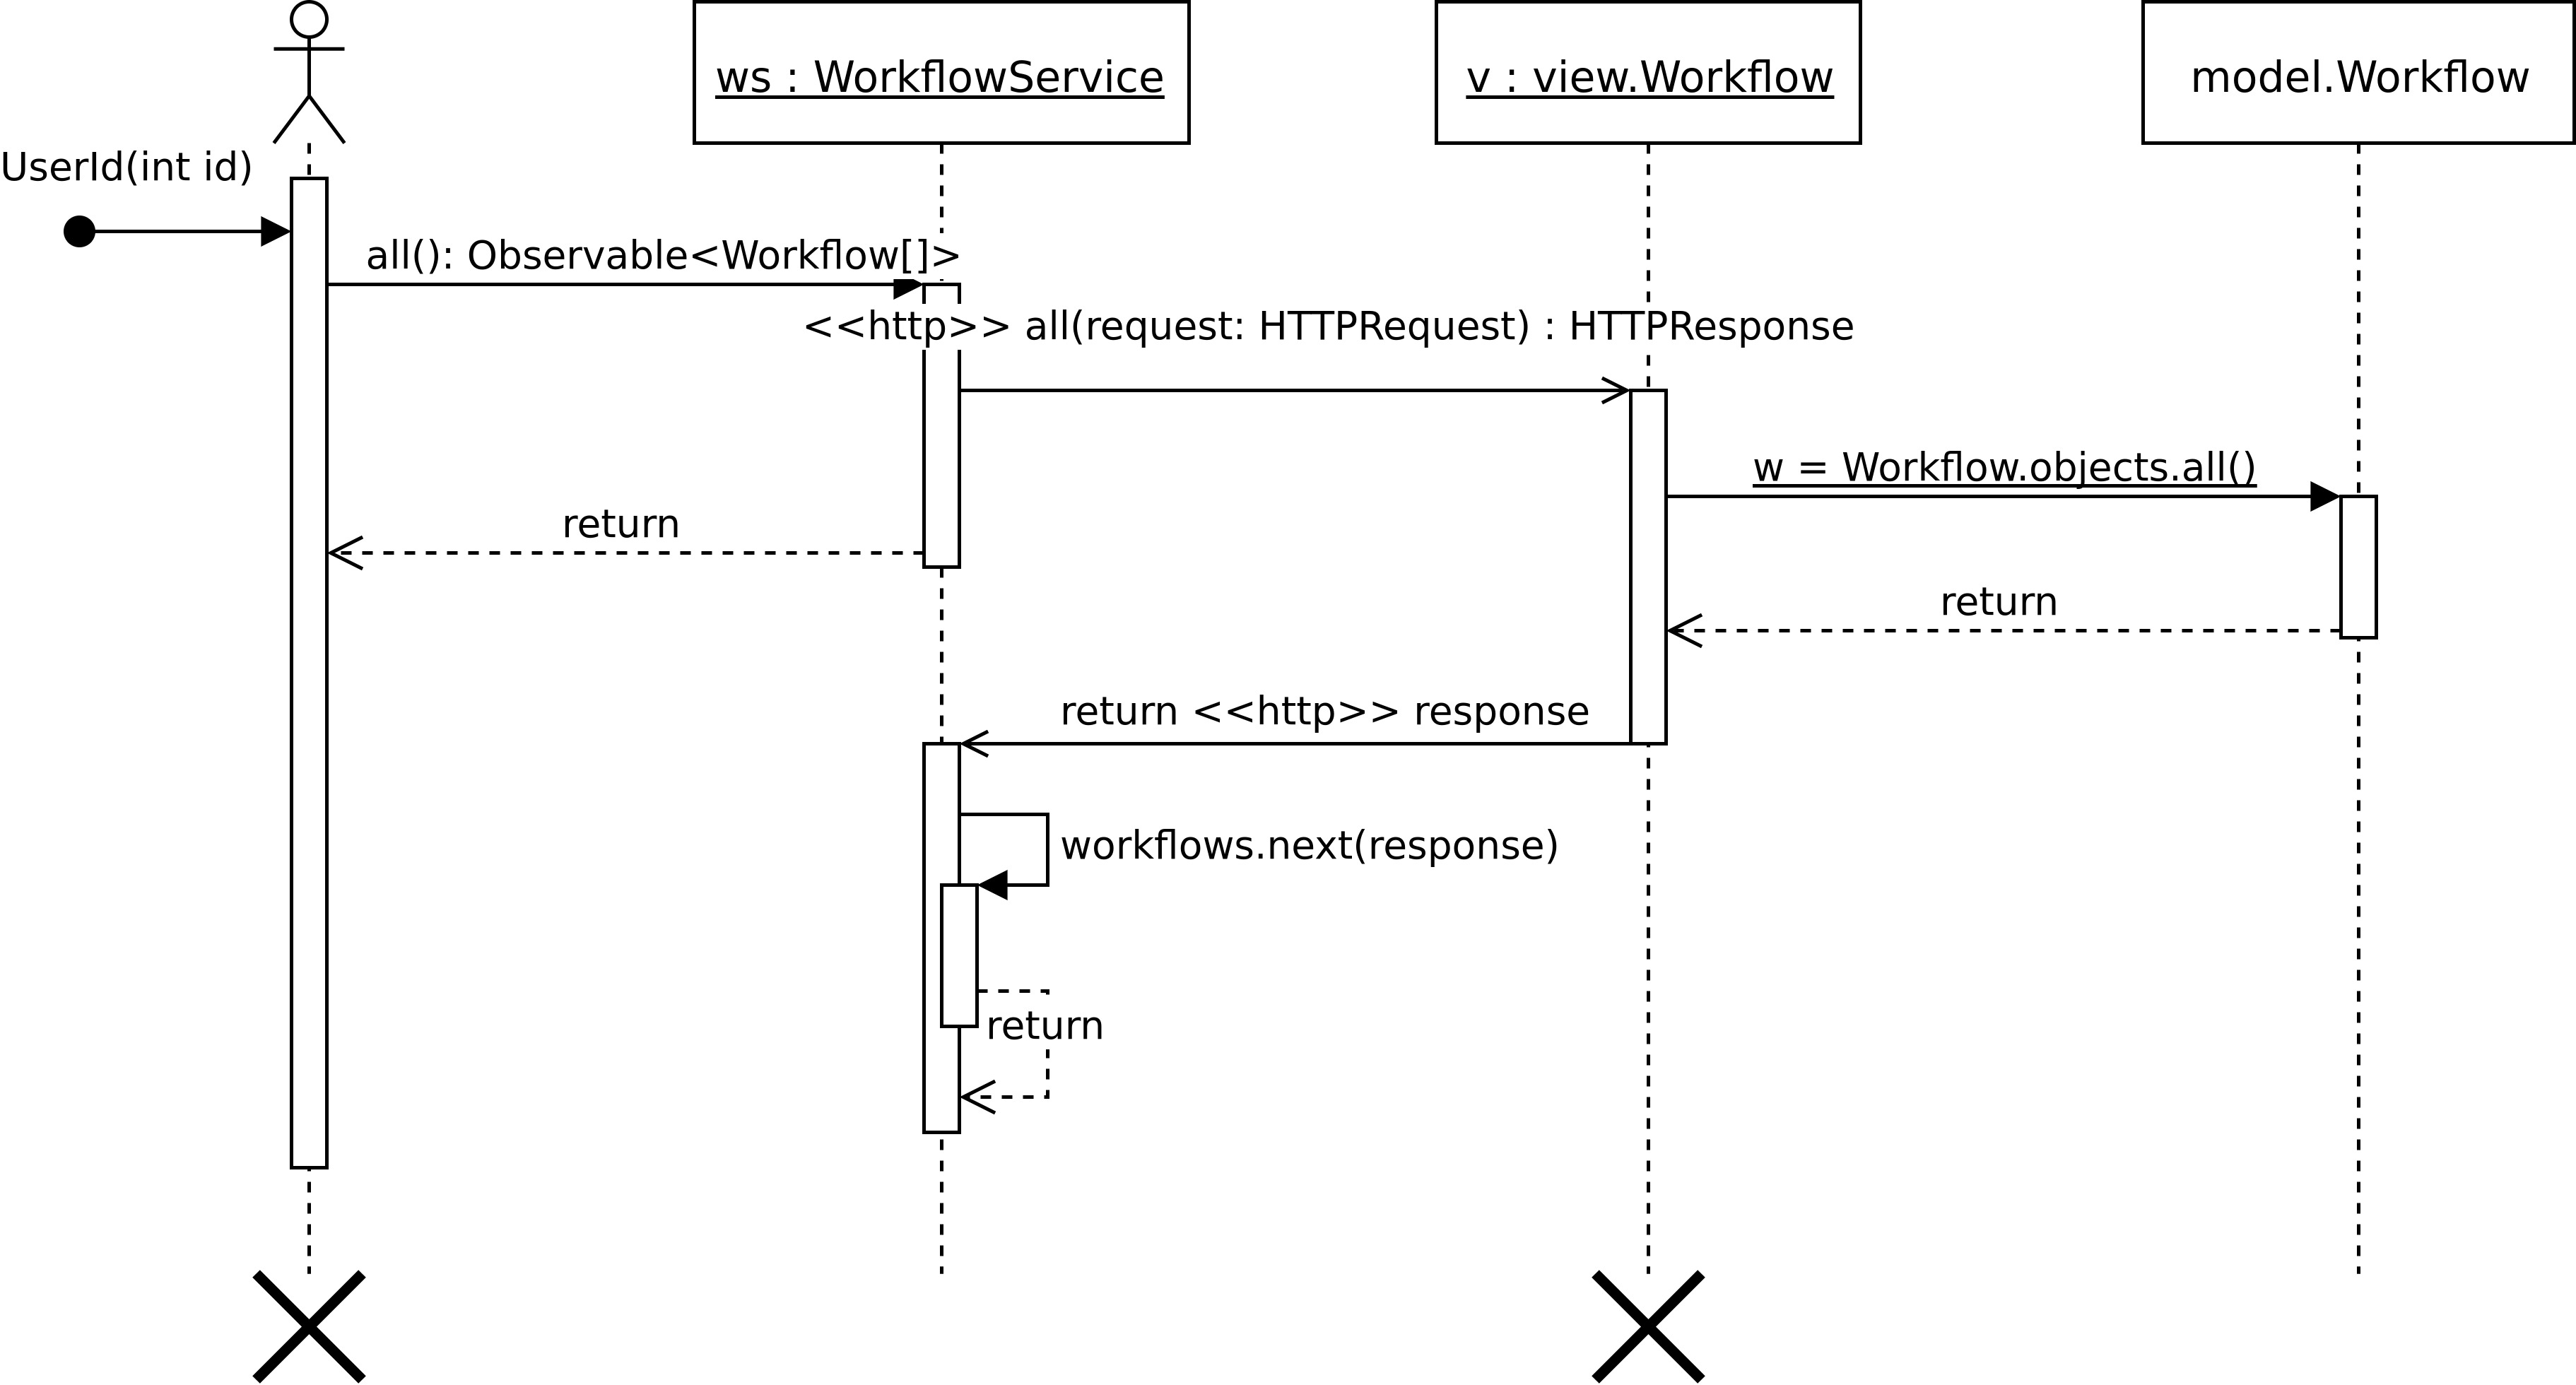
\includegraphics[width=15cm]{images/sqd_get_all_workflows.jpg}
        \caption{Get All Workflows}
        \label{sqd_get_all_workflows}
    \end{figure}
    
    \item     
    Bei \ref{sqd_get_workflow} verläuft das analog wie bei \ref{sqd_get_all_workflows}, mit der Ausnahme, dass hier entsprechenden immer nur ein Workflow anhand seiner ID geladen wird. Hier wird u.a. ebenfalls der aktuelle Ausführungsstatus des Workflows geladen.
    
    \begin{figure}[h]
        \centering
        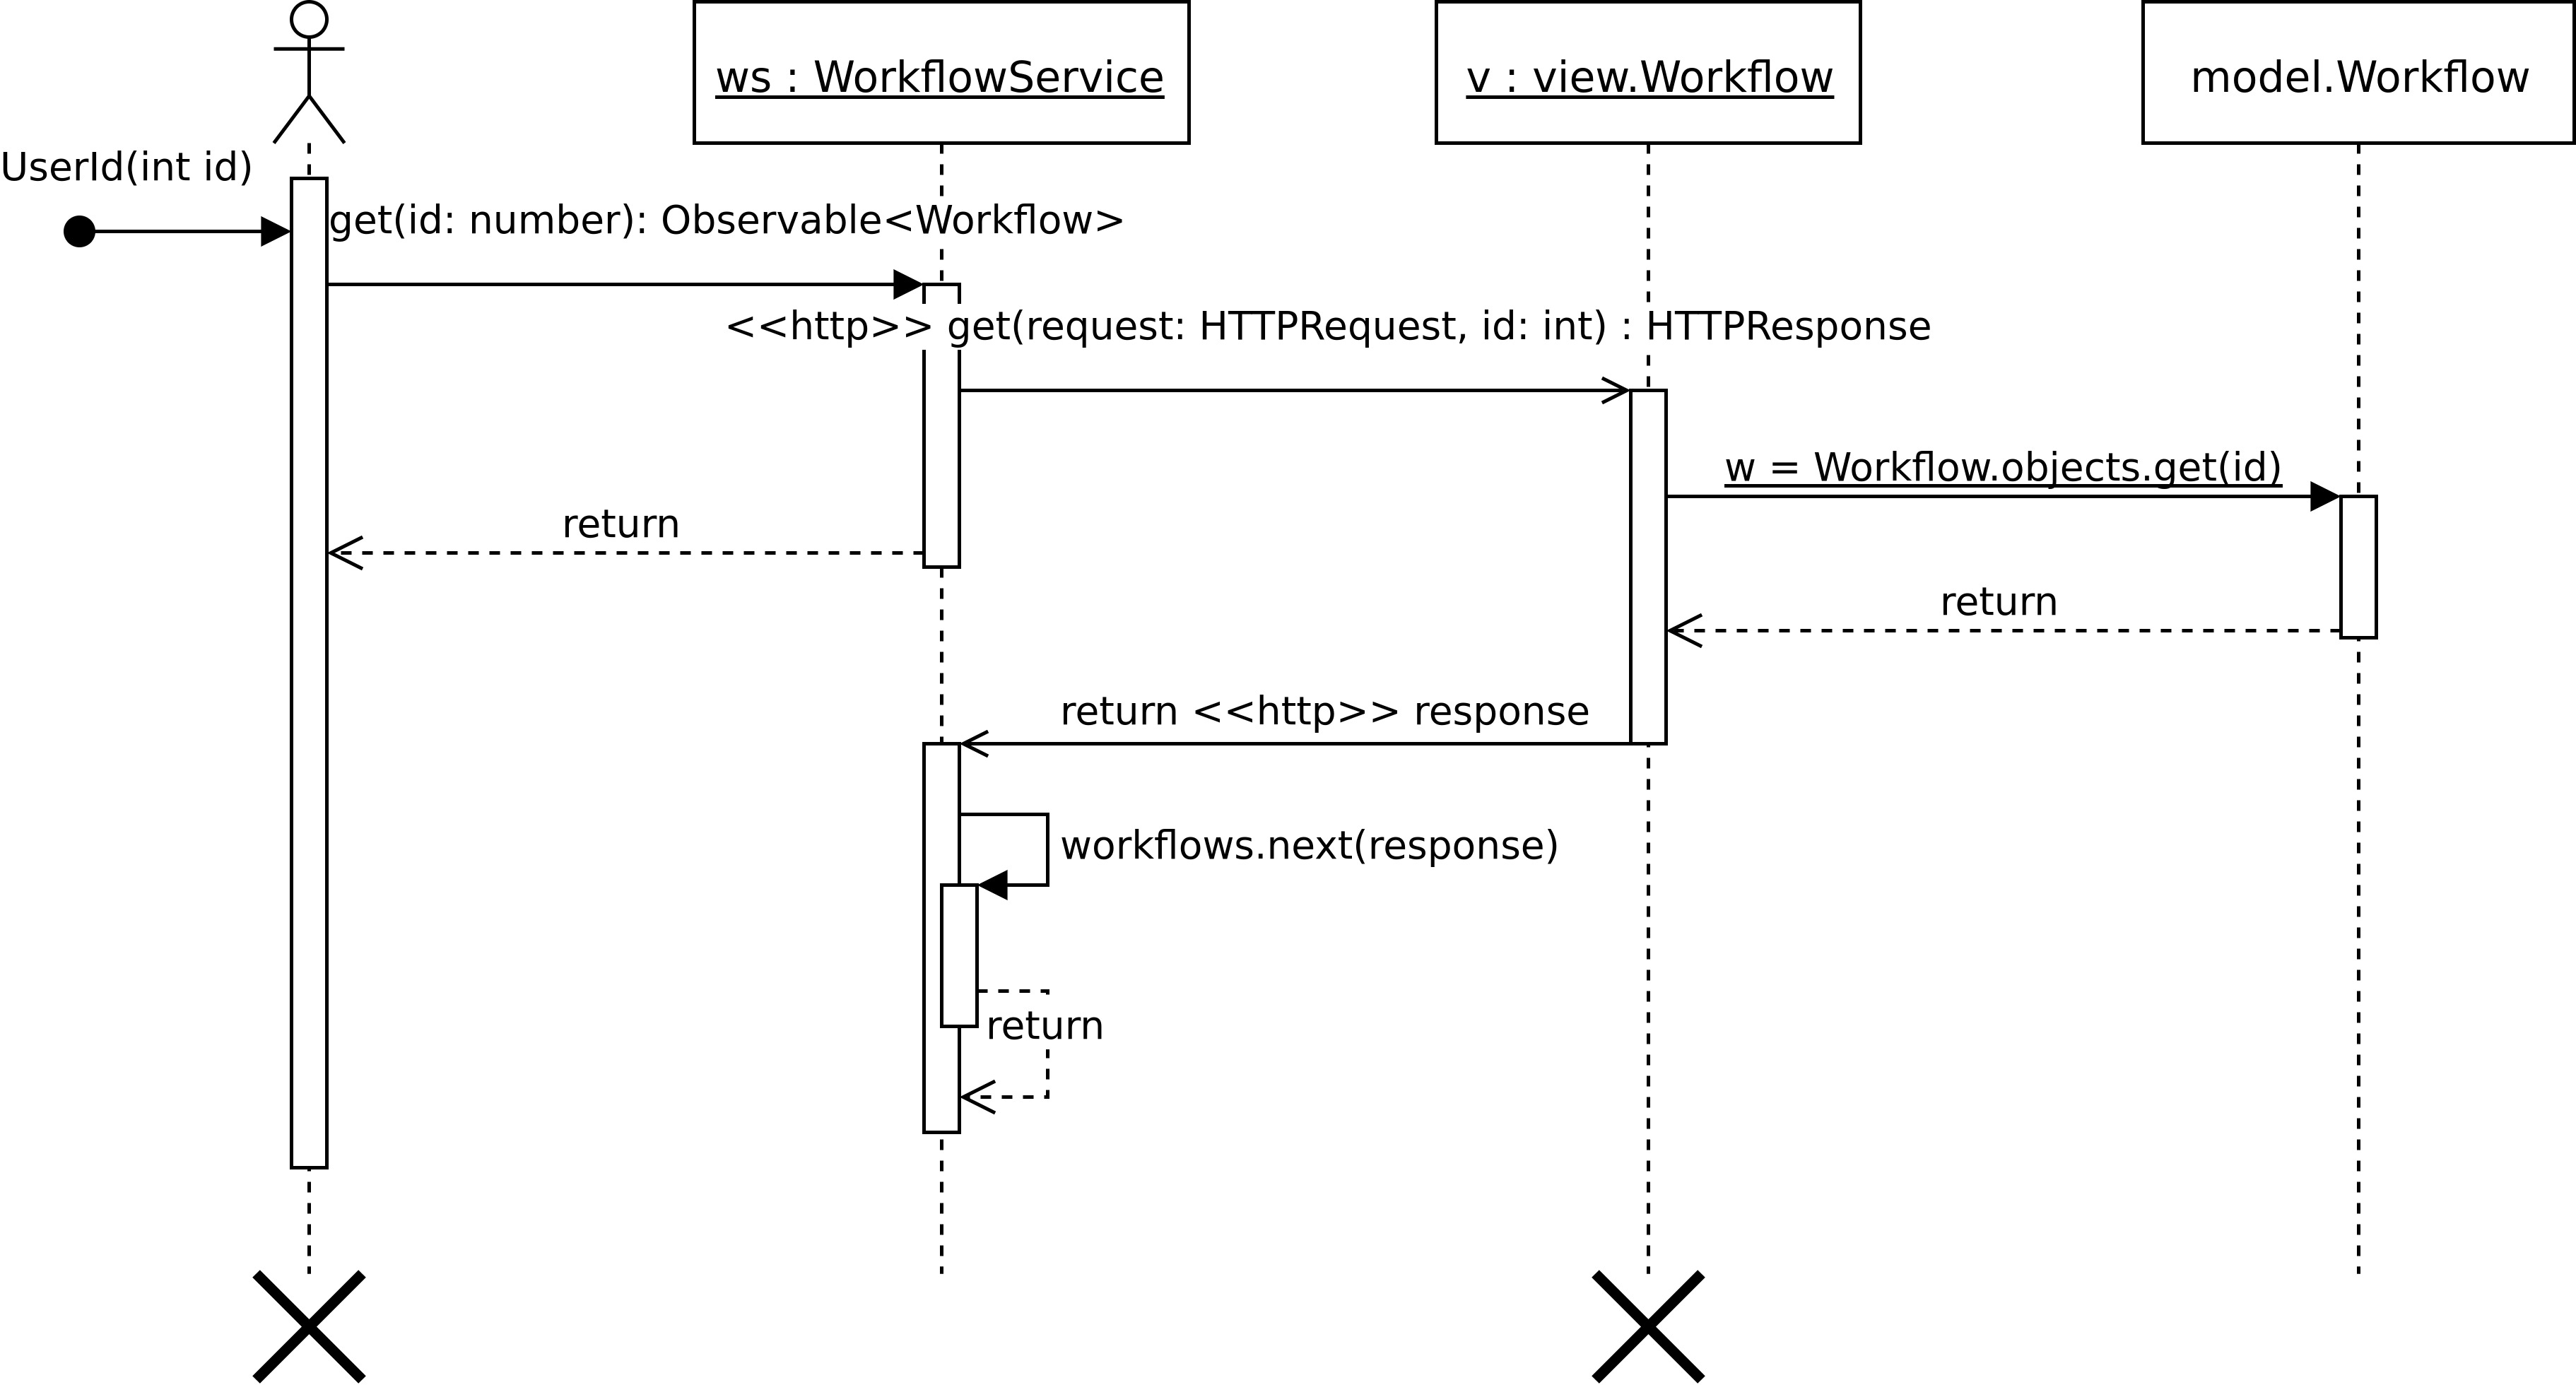
\includegraphics[width=15cm]{images/sqd_get_workflow.jpeg}
        \caption{Get Workflow}
        \label{sqd_get_workflow}
    \end{figure}
    
    \item
    Der Benutzer ist bereits mit seiner eindeutigen User ID eingeloggt und hat einen Workflow geladen. Der Benutzer will den Workflow als neuen Workflow speichern. Er drückt auf "speichern", hier wird er aus dem Editor auf WorkflowService mittels der create(workflow) Methode geleitet. Diese sendet einen HTTP Request an view.Workflow. Hier wird dann serverseitig ein neuer Workflow in der Datenbank angelegt. Danach gibt es einen HTTP Response zurück zum WorkflowService. Dies geht analog um einen neuen leeren Workflow zu kreieren, nur das hierbei nicht ein bereits vorhander Workflow gespeichert oder gar geladen sein muss. 
    
    \begin{figure}[h]
        \centering
        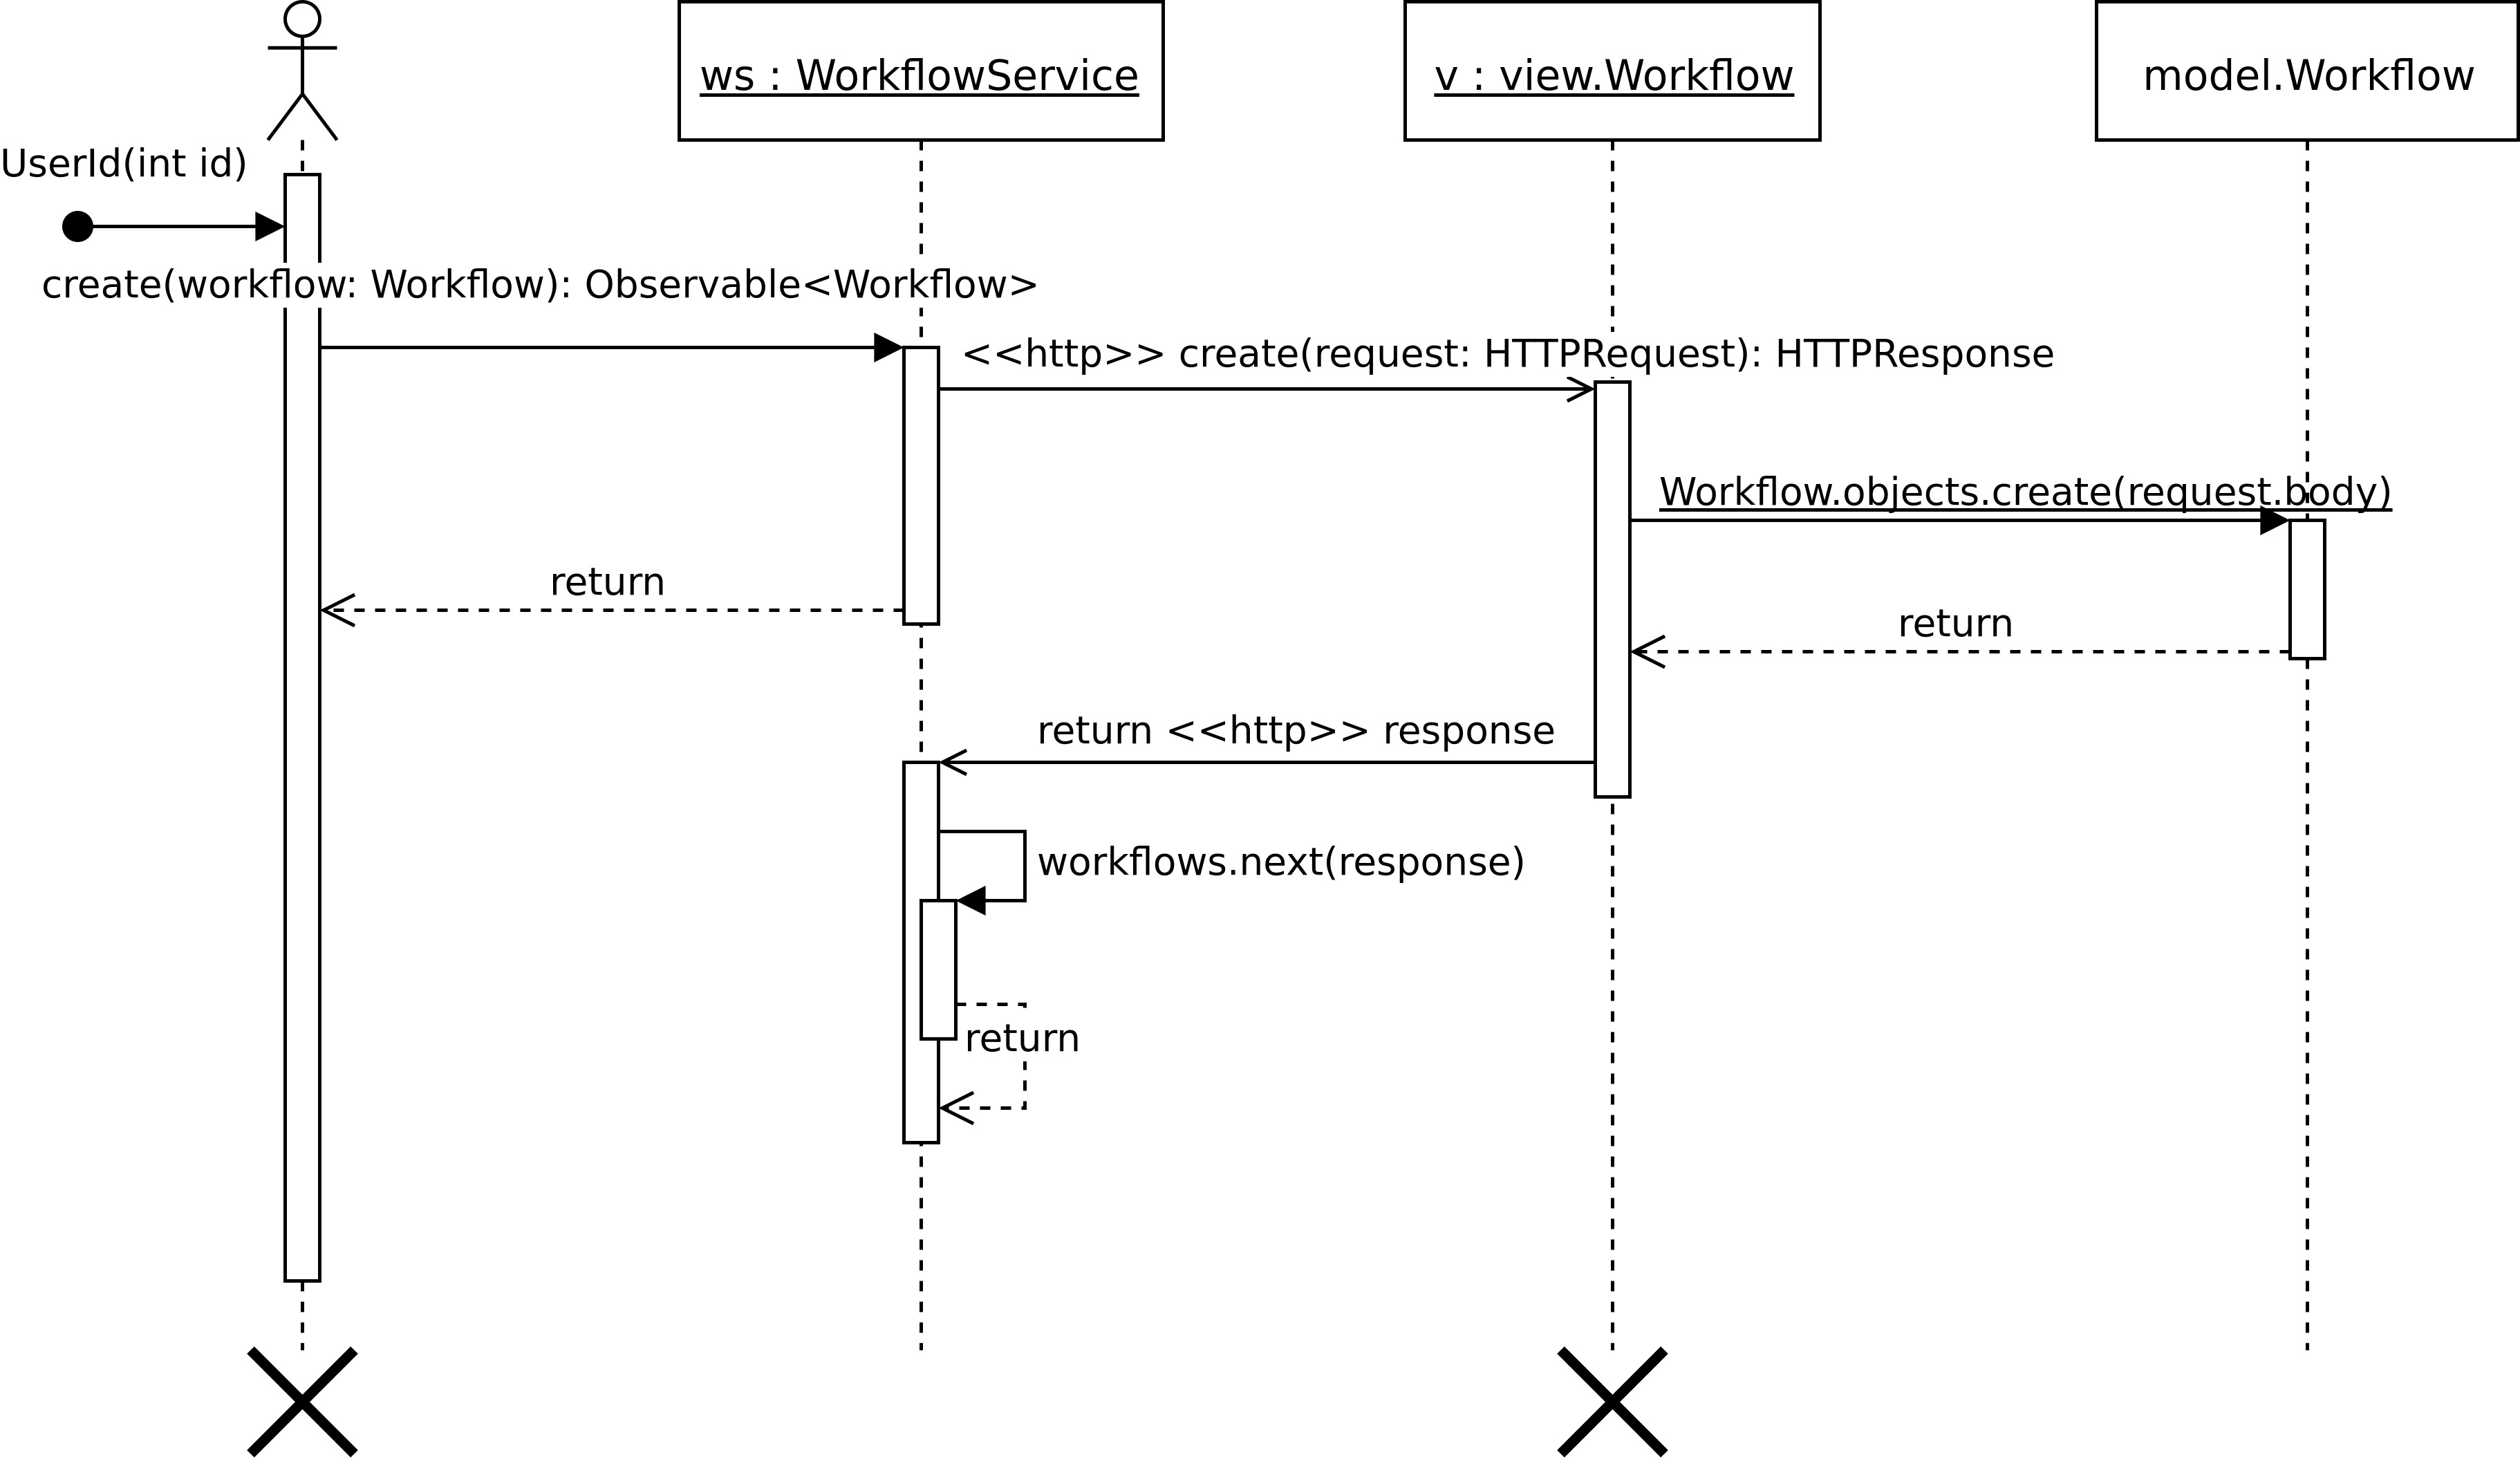
\includegraphics[width=15cm]{images/sqd_save_workflow.jpeg}
        \caption{Save Workflow / Create new Workflow}
        \label{sqd_save_workflow}
    \end{figure}
    
    \item 

\end{itemize}
